\chapter{Testing Framework}
Im folgenden Kapitel wird auf die einzelnen Komponenten des Test Frameworks eingegangen und deren Funktionsweise erläutert. Die Aufgabe des Test Frameworks liegt darin, die verschiedenen Prototypen, welche im Laufe dieser Semesterarbeit entwickelt wurden, mit diesem Framework einheitlich testen zu lassen. Das Test Framework wurde parallel zum RMIOnly- Systems mit Concurrency Control entwickelt.

\section{Konzept}
Das Framework lässt sich über eine Konfigurationsdatei konfigurieren und kann Testfälle, welche in einer XML Datenstruktur vorliegen, intepretieren und daraus die einzelnen Testszenarien generieren. Die Testszenarien werden vom Server auf die verfügbaren Testframework Clients verteilt und dort gestartet. Das Framework startet das zu testende System auf den verschiedenen Rechnern, welches unmittelbar danach die Aktionen durchführt, welche im übergebenen Szenario definiert wurden.\newline
Die mit den Messwerten ausgefüllten Szenarien werden an den Server zurück\-geschickt und dort ausgewertet. Dies ermöglicht einen Vergleich der verschiedenen eingesetzten Algorithmen. Folgende Eckpunkte muss das Framework erfüllen:

\begin{itemize}
\item Die enwickelten Sys\-te\-me müssen sich ohne Programmcode- Anpassungen an das Framework anbinden lassen
\item Das Framework muss die genauen Zeiten, welche für die Ausführungen der Operationen nötig waren, messen können
\item Nach einem Testlauf muss ein Bericht erstellt werden können, welcher die nötigen Informationen darstellt
\end{itemize}

\section{Allgemeine Informationen}
\label{sec:allgInformationen}

Um möglichst genaue Messdaten zu erlangen, wird das ganze System nach einem Testlauf beendet. Eine Aneinanderreihung von verschiedenen Test\-läufen würde die Messdaten aufgrund der JavaVirtualMachine be\-ein\-träch\-ti\-gen. Es besteht die Möglichkeit, dass für einen zweiten Testlauf weniger Speicher zur Verfügung steht, weil der Speicher immer noch mit Objekten des ersten Testlaufs besetzt ist. Da dies nicht mit Sicherheit überprüft werden kann, daher es kann nicht gewährleistet werden, dass die Grundvoraussetzungen für beide Testläufe gleich sind, wurde auf eine Aneinanderreihung von Testläufen verzichtet.

\section{Open Points (TODO's)}
\begin{itemize}	
\item Netzwerk Traffic der im Zimmer Auftritt kann nicht kontrolliert werden. Messungen daher nicht verlässlich, man bäuchte ein eigenes Netz.
\item JVM Profiler: Beweis für die Zombie Objekte in der JVM, soll das gemacht werden?
\item Exception Handling
\end{itemize}


\section{Der Frameworkserver}
\label{sec:test-FW Server}
\subsection{Das Startup-Script}
\label{sec:startupScript}
Das  Startup-Script ist ein Shell-Script in der Bash-Sprache geschrieben. Das Script führt mehrere Methoden nacheinander aus:
\begin{enumerate}
\item Ein ant- Script wird an\-ge\-stos\-sen, wel\-ches die Pro\-jek\-te kom\-pi\-liert. Durch die\-sen Schritt ent\-stehen die .jar- Dateien, welche im nächs\-ten Schritt benötigt werden
\item Das Script prüft die in der Config-Datei eingetragenen Zielrechner auf bereits vorhandene "client.jar"-Dateien und löscht diese Dateien, falls vorhanden
\item Durch die Applikation "Secure Copy" wird die zuvor im Buildprozess erstellte Datei "client.jar" auf die Zielrechner kopiert
\item Via SSH wird der Frameworkclient auf den Zielrechnern gestartet
\item Der Frameworkserver wird gestartet
\end{enumerate}
Sind diese Schritte abgeschlossen, beendet das Startupscript und die weitere Ausführung des Testlaufs wird durch den Frameworkserver orchestriert.
Beim Starten des Scripts wird der Name der Datei mitgegeben, in welcher der genaue Testlauf definiert ist. Wird kein Argument mitgegeben, läuft der Standardtestlauf ab, welcher in der Datei "testCases.xml" beschrieben ist.
Probleme beim Schreiben des Scripts waren selten. Ein Problem, welches gelöst werden musste war der Umstand, dass das Script nach dem Starten eines Clients nicht mehr weiterlief, sondern einfach wartete. Dies war bei folgende Zeile der Fall:
\begin{lstlisting}[breaklines=true]
 ssh student@${i} "java -jar ${remotePath}/${clientJar}"
\end{lstlisting}	
Offensichtlich wartet das Script beim Ausführen eines Befehls auf einem fremden Rechner auf einen Rückgabewert in irgendeiner Form; also auf einen Errorcode oder aber auf einen Exitstatus. Das Absetzen dieses Befehls musste also in einem seperaten Kind-Prozess stattfinden, damit der Eltern-Prozess die weiteren Aufgaben des Scripts abarbeiten konnte und nicht auf einen Rückgabewert wartete. Dies kann in der Bash-Shell mit einem "\&" erreicht werden. Die simple Lösung des Problems sieht also fast gleich aus:
\begin{lstlisting}[breaklines=true]
 ssh student@${i} "java -jar ${remotePath}/${clientJar}" &
\end{lstlisting}

\subsection{Startprozess des Frameworkservers}
\label{sec:startFramework}
In diesem Kapitel werden die Schritte beschrieben, welche vor dem Starten des Testlaufs durchgeführt werden. Der Frameworkserver, einmal gestartet, administriert den ganzen weiteren Ablauf des Testlaufs. \newline
Die Kommunikation des Frameworkservers mit den Frameworkclients ist in folgendem Sequenzdiagramm grob dargestellt:


\begin{figure}[H]
\begin{center}
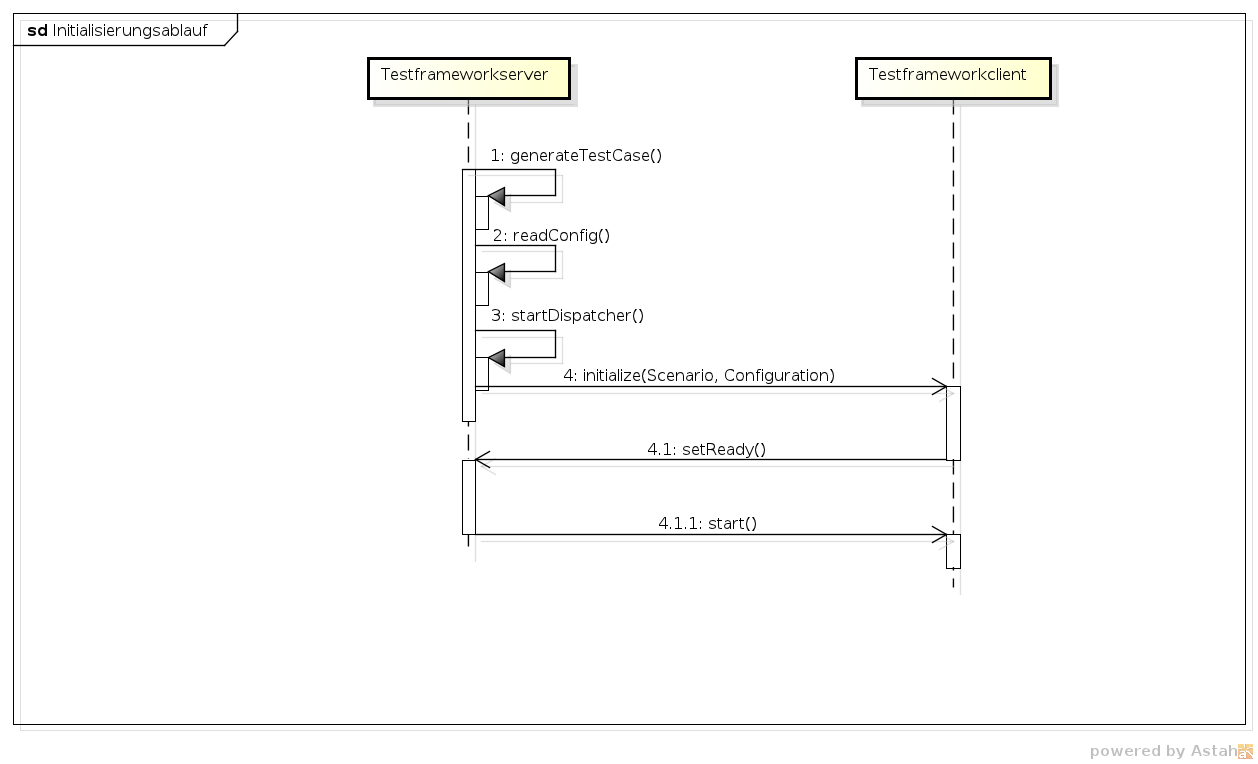
\includegraphics[scale=0.3]{image_testFramework/TestFWInit.png}
\end{center}
\caption{Testframework Init}
\end{figure}

Die im Diagramm dargestellten Operationen lassen sich wie folgt erklären:

\begin{itemize}
\item Die Methode generateTestCase() ruft eine Factory auf, welche aus einer XML-Datei einen Testcase generiert. Diese Factory wird unter dem Ka\-pi\-tel Testcase-Factory genauer be\-schrie\-ben.
\item Alle Konfigurationsparameter welche der Server braucht, sind in einer Konfigurations\-datei ab\-ge\-legt. Durch eine Configurationfactory wird durch mit Hilfe der Konfig\-urationsdatei ein Configuration- Objekt er\-zeugt. Unter dem Kapi\-tel "Configuration-Factory" wird dies näher beschrieben.
\item Nachdem die Konfigurationsparameter ausgelesen wurden, kann der Dis\-patcher in einem seper\-aten Thread ge\-startet werden. Weitere Aus\-füh\-run\-gen sind unter dem Kapitel "Der Dispatcher" zu finden.
\item Bei der Initialisierung der Clients, wird diesen je ein Scenario und ein Configuration-Objekt gesendet. Das Configuration-Objekt umfasst alle für den Client wichtigen Konfigurationsparameter, wie etwa die Ports, unter welchen der Server seine Dienste zur Verfügung stellt. Was ein Scenario genau ist wird unter dem "Kapitel Testcase-Factory" genauer beschrieben.
\item Pro Client hat der Server beim Auslesen der Konfigurationsdatei ein Client-Objekt instanziert. Dies wurde voral\-lem zur Kon\-trol\-le der Cli\-ents durch den Server so implementiert. Darauf wird im Kapitel "ClientObjekt" eingegangen.
\item Nachdem alle Clients "setReady()" aufgerufen haben, ruft der Server "start()" auf allen Clients auf. Dieser Vorgang wird unter dem Punkt "die Start-Methode" genauer erläutert.
\end{itemize}

\subsubsection{Testcase-Factory}
\label{sec:testCaseFactory}
Die Testcase-Factory liest ein XML-File, in welchem ein sogenannter "TestCase" definiert ist. Wird beim Starten des Frameworkservers kein Paramter mitgegeben, wird der Standard-Testcase gewählt, welcher in der Datei "testCases.xml" abgelegt ist. Wird aber ein Parameter mitgegeben, beschreibt dieser den Namen der auszuführenden TestCase-Datei.\newline
Durch die ein\-ge\-lesenen In\-for\-ma\-tio\-nen er\-stellt die Fac\-tory die Szena\-rien, wel\-che dann wei\-ter an die ver\-schie\-denen Clients ge\-sendet werden. Folgender Block ist ein Auszug aus einer TestCase-Datei:

\begin{lstlisting}[language=XML, breaklines=true] 	
<?xml version='1.0' encoding='UTF-8'?>
<TestRun>
  <TestCase SystemUnderTest="ch.hsr.objectCaching.rmiOnlyClient.RMIonlyClientSystem">
    <Account balance="1"></Account>
      <Scenario id="1">
        <ActionSequence>
          <Increment count ="100" delay="0" factor="1.1"></Increment>
	</ActionSequence>
      </Scenario>
      <Scenario id="2">
	<ActionSequence>
          <Increment count ="100" delay="0" factor="1.1"></Increment>
	</ActionSequence>
      </Scenario>
  </TestCase>
</TestRun>
\end{lstlisting}

Das Attribut "SystemUnderTest" definiert das zu testende System. Der Vorteil dieser Methode ist, dass das zu testende System einfach in XML angegeben wird und dann getestet werden kann. Es müssen also keine Anpassungen am Code vorgenommen werden, egal welches System getestet werden soll. Dem Framework ist es schlussendlich egal, welches System getestet werden soll.\newline
Eine TestCase-Datei beschreibt genau einen TestCase. Ein Test\-Case kann ver\-schie\-dene Sze\-na\-ri\-en be\-in\-hal\-ten, oder aber auch nur ein Szena\-rio be\-schrei\-ben. Ist nur ein Sz\-enario definiert, werden beide Clients mit dem\-selben Szenario arbeiten. Falls mehrere Szenarien beschrieben sind, werden die Clients unterschiedliche Szenarien durchführen. \newline
Aus obigem XML-Code generiert die Factory nun ein Objekt vom Typ TestCase. Dieses Objekt definiert nun zwei Szenarien, welche wiederum aus mehreren Actions bestehen. Was genau eine Action ist, ist unter dem Kapitel "Actions" beschrieben. Die Factory wird nun bei diesem Beispielcode eine Abfolge von 100 "Increment-Action" erstellen und diese in das Scenario-Objekt ablegen.


\subsubsection{Configuration-Factory}
\label{sec:configurationFactory}
Die Configuration-Factory liest alle Daten aus der Konfigurationsdatei aus und erstellt mit diesen Informationen ein Configuration-Objekt. Die Konfigurationsdatei sieht wie folgt aus:
\begin{lstlisting}
Client0=152.96.193.18
Client1=152.96.193.19
Clientport=36927
ServerRmiPort=36925
ServerSocketPort=36926
ServerRegistryName=Server
ClientRegistryName=Client
\end{lstlisting}

In der Konfigurationsdatei ist definiert, welche Clients auf welchem Port kontaktiert werden können. Weiter ist der Registry-Name definiert, damit der Server weiss, über welche Registry er die Methoden auf dem Client aufrufen muss. \newline
Aus diesen Informationen erstellt die Factory ein Configuration- Objekt, welches sie dem Client als erstes sendet. Damit ist gewährleistet, dass der Frameworkserver und die Frameworkclients miteinander über RMI kommunizieren können. \newline
Pro Client, welcher hier definiert ist, wird ein Client-Objekt instanziert, was im folgenden Kapitel beschrieben wird.

\subsubsection{ClientObjekt}
\label{sec:ClientObjekt}

Das Clientobjekt besitzt unter anderem ein Datenfeld, welches genau zwei Zustände annehmen kann: Ready und NotReady. Führt der Frameworkclient die Methode "setReady()" auf dem Server aus, wird der Status auf dem jeweiligen Objekt auf Ready gesetzt. Folgend die Implementation der setReady-Methode:
\begin{lstlisting}[language=Java, breaklines=true]
public void setReady(String ip) 
{
	logger.info("Setted ready with: " + ip);
	Client temp;
	if((temp = clientList.getClientByIp(ip)) != null)
	{
		temp.setStartingState(StartingState.READY);
	}
	if(checkAllReady())
	{
		start();
	}
}
\end{lstlisting}

Interessant an dieser Methode ist die Funktion der "checkAllReady"-Methode. Dieser Mecha\-nismus ist nicht nur dazu da, um alle Clients mög\-lichst gleichzeitig zu starten, sondern auch, um die Threads zu steuern. Die Methode setReady() wird durch mehrere verschiedene Threads aufgerufen, von jedem Client genau ein Mal. Durch die Implementation von checkAllReady() wird aber nur der letzte Thread, welcher setReady() aufruft, weiterleben und start() ausführen können. Somit ist garantiert, dass auch danach nur ein Thread aktiv ist und keine Seiteneffekte entstehen können.\newline
Die Implementation dieser Logik war nicht schwer, doch das Bewusstsein für die Problematik mit mehreren Threads muss ständig vorhanden sein. Die Einflüsse der parallelen Programmierung stellten ohnehin einen spannenden Aspekt dieser Arbeit dar. 

\subsubsection{Die Start-Methode}
\label{sec:startMethode}

Die Methode "start()", gibt dem Client an, mit der Abarbeitung des Szenarios zu beginnen. Die erste Implementation dieser Methode sah wie folgt aus:
\begin{lstlisting}[language=java, breaklines=true]
private void start()
{
	logger.info("Method start() invoked");
	for(int i = 0; i < clientList.size(); i++)
	{
		clientList.getClient(i).getClientStub().startTest();
	}
}
\end{lstlisting}

Nach einigen Testdurchläufen konnte festgestellt werden, dass die Clients ihre Szenarien nur sequentiell abarbeiteten und die Operationen auf dem Server nicht gleichzeitig geschehen. Schuld an diesem Umstand war obige Implementation der "start"-Methode. Der Server-Thread, welcher "startTest()" auf dem Client aufrief, wartete solange, bis die Methode zurückkehrte. Da die Methode natürlich erst nach der Beendigung des Szenarios zurückkehrt, konnte nur immer genau ein Client zu einem gewissen zeitpunkt aktiv sein.\newline
Die jetzige Implementation und somit die Lösung des Problems sieht wie folgt aus:
\begin{lstlisting}[language=java, breaklines=true]
private void start()
{
	logger.info("Method start() invoked");
	for(int i = 0; i < clientList.size(); i++)
	{
		ClientStart clientStart = new ClientStart(clientList.getClient(i));
		new Thread(clientStart).start();
	}
}
\end{lstlisting}
Um das Problem mit der Erstellung eines neuen Threads für jeden zu startenden Client zu umgehen, musste eine weitere Klasse Namens ClientStart ge\-schrie\-ben wer\-den. Die Klas\-se im\-p\-le\-men\-tiert natür\-lich das Inter\-face "Run\-nable" und im\-p\-le\-men\-tiert die "run()"-Methode wie folgt:
\begin{lstlisting}[language=java, breaklines=true]
public void run() {
	try {
		client.getClientStub().startTest();
	} catch (RemoteException e) {
		logger.log(Level.SEVERE, "Uncaught exception", e);
	}
}
\end{lstlisting}

Mit dieser Implementation wird der Methodenaufruf "start()" nun von einem seperaten Thread ausgeführt. Dies führt dazu, dass die Clients nun zeitlich parallel gestartet werden und nicht nacheinander. Da die einzelnen Threads nach Beendigung der "run()"-Methode sterben, ist die Art der Implementation unbedenklich bezüglich Seiteneffekte oder "zombie-Threads".

\subsubsection{Der Dispatcher}
\label{sec:dispatcher}

Der Dispatcher stellt die Verbindung zwischen dem Frameworkserver und dem Server des Systems, welches getestet werden soll, dar. Dem Dispatcher wird die Portnummer angegeben, unter welcher er ein Socket öffnen soll. Weiter wird ihm ein String übergeben, in welchem der Pfad des zu testenden Systems drinnsteht. Der Dispatcher instanziert dann das zu testende System mit Hilfe des Strings und wartet dann in einem blockierten Zustand auf sich verbindende Clients. Nachdem ein Client auf dem geöffneten Socket eine Verbindung aufgebaut hat, übergibt der Dispatcher die Verbindung in Form eines Input und eines Outputstreams dem Server des zu testenden Systems.\newline
Logischerweise läuft der Dispatcher wiederum in einem seperaten Thread.

\subsection{Herunterfahren des Frameworkservers}
\label{sec:herunterfahrenFramework}

Nach Beendigung eines Testlaufs, muss der Server mehrere Arbeiten erledigen. Nachfolgend werden die wichtigsten Aufgaben, welche der Server nach einem Testlauf erledigen muss, aufgeführt:


\begin{figure}
\begin{center}
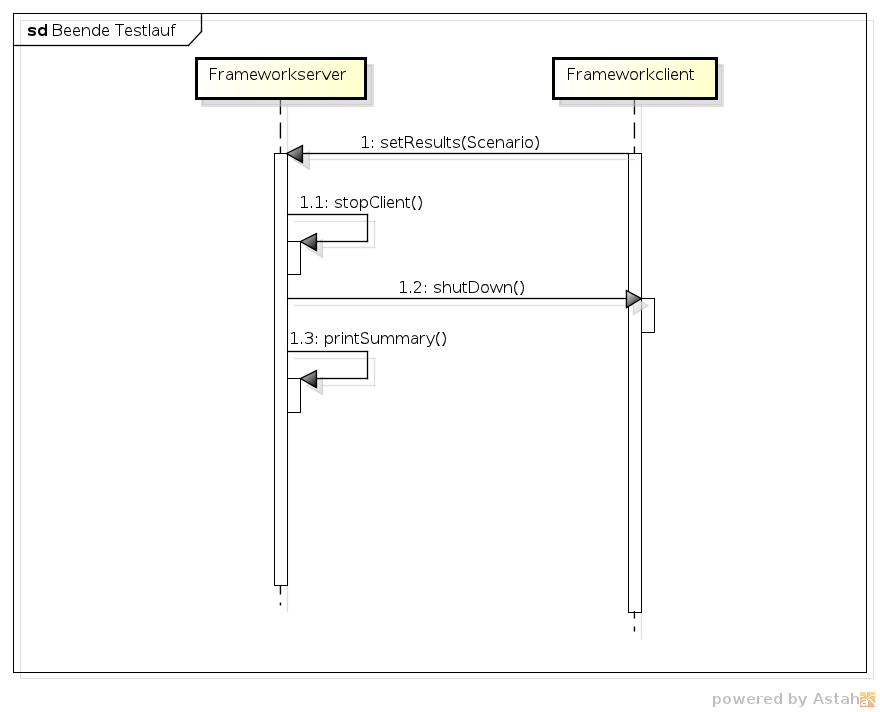
\includegraphics[scale=0.2]{image_testFramework/BeendeTestlauf.png}
\end{center}
\caption{Testfamework Exit}
\end{figure}

Die im Diagramm ersichtlichen Operationen können folgender\-massen er\-läu\-tert werden:
\begin{itemize}
\item Die Methode "setResults(Scenario)" wird vom Client auf dem Server auf\-ge\-rufen. Durch den Aufruf dieser Methode weiss der Server, dass der aufrufende Client sein Szenario durchgespielt hat. Weiter wird mit dem Aufruf der Methode wiederum ein Thread durch den RMI-Daemon gestartet, welcher die weiter folgenden Methoden anstösst.
\item Aus der "setResults(Scenario)"- Methode wird di\-rekt "stopClient()" auf\-ge\-rufen. Was diese Methode genau macht, wird im Kapitel "Stoppen eines Clients" genau beschrieben.
\item Die Methode "shutDown()" wird auf dem Client aufgerufen. Der Client trennt daraufhin die RMI-Verbindung zum Server und schaltet sich selber ab. Nähere Informationen zum Abschaltungsprozess eines Clients kann unter dem Kapitel "Testframework Client" nachgelesen werden.
\item Die Methode "printSummary()" verwertet die Ergebnisse, welche die Clients in ihrem Szenario gespeichert und wieder übertragen haben. Mehr Informationen dazu im Kapitel "Report Generator". Weiter wird auf der Console ausgegeben, ob es "Lost-Update"-Probleme gegeben hat oder nicht. Mehr zu diesem Thema unter "Result Generator".
\end{itemize}

\subsubsection{Stoppen eines Clients}
\label{sec:stopClient}
Ruft ein Client die Methode "setResults(Scenario)" auf dem Server auf, wird Serverintern der Status des Clients auf "Down" gesetzt. Da die Methode "stopClient()" wiederum pro Client genau ein Mal aufgerufen wird, entsteht wieder das Problem, dass mehrere Threads am Leben sind. Um dies ab einem gewissen Punkt zu verhindern, wurde ähnlich zur "setReady()"-Methode, folgende Implementation gewählt:
\begin{lstlisting}[language=java, breaklines=true]
private void stopClient(String clientIp)
{
	Client temp;
	try {
		
		if((temp = clientList.getClientByIp(clientIp)) != null)
		{
			logger.info("stop client with ip: " + clientIp);
			temp.setClientRunning(ShutedDown.DOWN);
			temp.getClientStub().shutdown();
		}
	} catch (RemoteException e) {
		logger.log(Level.SEVERE, "Uncaught exception", e);
	}
	if(checkAllShutedDown())
	{
		printSummary();
	}
}
\end{lstlisting}

Durch die Prüfung "checkAllShutedDown()", wird nur der letzte aller Threads weiterleben. Somit wird auch nur ein Thread fähig sein die Methode "printSummary()" auszuführen, während die anderen Threads die Methode zu Ende abarbeiten und am Ende der Methode sterben. Durch diese Implementation wird sichergestellt, dass nur ein Thread weiterlebt und keine "Zombi-Prozesse" mehr vorhanden sind.\newline
Weiter wird beim Abarbeiten dieser Methode die Methode "shutdown()" auf dem Client aufgerufen. Nach diesem Aufruf fährt sich der Client herunter und kappt alle akiven Verbindungen zum Server. Weitere Informationen zum Shutdown-Prozess des Clients sind unter der Kapitel des Frameworkclients ersichtlich.\newline
Oben genannte Implementation der "stopClient(String clientIP)"-Methode hat lange funktioniert. Während des Entwicklungsprozesses der RMI-Only Lösung lief das Framework mit der erwähnten Methode ohne Probleme. Bei den ersten Testläufen der RMI-Cache Lösung wurden beim Herunterfahren der Umgebung allerdings Exceptions generiert. Da die Fehlersuche bei Software mit einer vielzahl von Threads sehr langwierig ist, dauerte die Analyse des Fehlers relativ lange.\newline Schlussendlich wurde bemerkt, dass die Methode "printSummary()" trotz aller Vorsichtsmassnahmen von jedem Client ein Mal ausgeführt wurde, was dazu führte, dass mehrere Zusammenfassungen generiert wurden und probiert wurde, den FrameworkServer mehrere Male herunterzufahren. Der Versuch den FrameworkServer mehrmals herunterzufahren war natürlich der Grund für die Ex\-cep\-tions, da dem zweiten Client ein\-fach der Ver\-bin\-dungs\-part\-ner weggerissen wurde.\newline
Der Grund des Fehlverhaltens lag in der nicht funktionierenden Barriere "checkAllShutedDown()". Nachdem der Methodenkopf durch snychronized erweitert wurde, funktionierte das Framework wieder problemlos:
\begin{lstlisting}[language=java, breaklines=true]
synchronized private void stopClient(String clientIp)
\end{lstlisting}
Anscheinend sind die Clients bei der Cache- Implementation immer zum fast gleichen Zeit\-punkt fer\-tig, was dazu führte, dass der Sta\-tus "ShutedDown.DOWN" nur un\-zu\-ver\-läs\-sig gesetzt wurde. Das Fehlerszenario lief wie folgt ab:
\begin{itemize}
\item Thread1 betritt die "stopClient(String clientIp)"-Methode und setzt seinen Status auf DOWN
\item Kurz nachdem Thread1 seinen Status gesetzt hat, wird im die Res\-sour\-ce entzogen und Thread2 kommt zum Zug
\item Thread2 betritt nun seinerseits die Methode und setzt seinen Status ebenfalls auf DOWN
\item Da nun alle Threads auf DOWN sind, wird die Barriere nicht mehr funktionieren und mehrere Threads führen "printSummary()" aus
\end{itemize}
Dadurch, dass die Methode nun synchronized ist, ist gewährleistet, dass sich nur ein Thread in der Methode aufhalten kann. Das wiederum bedeutet, dass die Barriere "checkAllShutedDown()" nun wieder funktioniert, da die Stati der Threads wieder zuverlässig gesetzt werden.

\subsubsection{Report Generator}
\label{sec:reportGenerator}

Wir die Methode "printSummary" aufgerufen, wird ein ReportGenerator instanziert, welche die Daten der Clients ausliest und in eine Textdatei schreibt. Folgende Werte wurden durch die Clients erfasst:
\begin{itemize}
\item Zeit, welche benötigt wurde um die entsprechende Action durch\-zu\-führen
\item Protokollierung, ob bei der Durchführung ein Konflikt generiert wurde oder nicht
\item Zeit, welche in einem Konfliktfall gebraucht wurde, um den Konflikt zu behandeln und die Operation noch einmal auszuführen
\end{itemize}

Pro Client wird eine Datei erstellt, in welcher die Daten dargestellt werden. Folgend einen kurzen Auszug eines solchen Reports:

\begin{lstlisting}[breaklines=true]
**************************************************
Result for Client: 152.96.193.18 with ScenarioID: 1
OS: Linux / 3.0.0-17-generic-pae
**************************************************
ActionNr;#ofTries;Time[ms];ACTION
0;0;42.674487;INCREMENT(READ) WITHOUT DELAY
0;1;77.969046;INCREMENT(WRITE) WITHOUT DELAY
1;0;79.684003;INCREMENT(READ) WITHOUT DELAY
1;1;81.984427;INCREMENT(WRITE) WITHOUT DELAY

------------------------------------------------
100% of all Action executed are successful
Total actions executed: 2, number of unsuccessful action 0
Total getBalance calls: 2, avg. execution time 61.179245
Total setBalance calls: 2, avg. execution time 79.9767365

Total Conflict: 0 / Gesamt Dauer: 282.311963 ms / durch. Dauer pro Operation: 141.1559815
\end{lstlisting}

Die genaue Messerwerte, mit Durch\-schnitts\-wer\-ten und Ver\-gleiche zwischen den verschiedenen Systemen sind am Schluss dieser Arbeit zu finden. \newline
Während der Entwicklung des Frameworks und der verschiedenen Systeme, schien die Ausgabe der Testergebnisse in eine Textdatei eine gute Idee zu sein. Während den Messungen des Systems wurde aber bemerkt, dass dies eine äusserst Zeitraubende und mühsame Arbeit nach sich zieht: Für einen Testcase mit acht Clients, bei welchem der Messgenauigkeit zu liebe drei Durchläufe getätigt werden, fallen insgesamt 24 Textdateien an. Um einen Mittelwert der Ergebnisse zu bekommen, müssen alle Textdateien geöffnet werden, die Mittelwerte müssen berechnet werden und in einer weiteren Datei abgelegt werden. \newline
Dieser Umstand wurde erst am Ende der Abrbeit bemerkt, weshalb auf eine aufwändie Lösung verzichtet wurde. Mögliche Lösungsansätze für dieses Problem:
\begin{itemize}
\item Die Ergebnisse werden in eine Datenbank geschrieben
\item Die Ausgabe erfolgt in ein XML-File
\end{itemize}
Die Ausgabe der Ergebnisse in eine Datenbank wäre wohl die sauberste Lösung, doch auch mit sehr viel Aufwand verbunden. Ein XML-File wäre sicher einfach zu handhaben, als die Textdateien und hätte schlussendlich weniger Aufwand für die Messungen bedeutet.

\subsubsection{Result Generator}
\label{sec:resultGenerator}
Der ResultGenerator ist ein Generator, welcher für die Berechnung des zu erwartenden Entbestandes des Account-Objektes verantwortlich ist. Wenn alle Clients ihre Operationen abgeschlossen haben, wird das aktuelle Ergebnis des Account-Objektes und das erwartete Ergebnis auf der Konsole ausgegeben. Zusätzlich wird kontrolliert, ob die Ergebnisse übereinstimmen und eine entsprechende Meldung wird auf der Konsole ausgegeben:
\begin{lstlisting}[breaklines=true]
19.04.2012 18:33:38 ch.hsr.objectCaching.testFrameworkServer.Server printSummary
INFO: AccountBalance is: 1.4641001269340557
19.04.2012 18:33:38 ch.hsr.objectCaching.testFrameworkServer.Server printSummary
INFO: AccountBalance should be: 1.4641001269340557
19.04.2012 18:33:38 ch.hsr.objectCaching.testFrameworkServer.Server printSummary
INFO: No Lost-Updates!
\end{lstlisting}

\subsubsection{Logger}
\label{sec:logger}
Wie in dem Konsolenauszug unter "Result Generator" gesehen werden kann, wurde ein Logger eingebaut, welcher alle Methodenaufrufe protokoliert. Der Logger schreibt die Ereignisse erstens auf die Konsole und zweitens schreibt er alle Informaionen zu einem Methodenaufruf in eine Datei. Diese Logdatei ist sehr Informationsreich:

\begin{lstlisting}[language=XML, breaklines=true]
<record>
  <date>2012-04-05T17:58:43</date>
  <millis>1333641523151</millis>
  <sequence>9</sequence>
  <logger>TestFrameWorkServer</logger>
  <level>INFO</level>
  <class>ch.hsr.objectCaching.testFrameworkServer.MethodCallLogger</class>
  <method>methodCalled</method>
  <thread>11</thread>
  <message>setBalance got invoked by /152.96.193.9</message>
</record>
<record>
  <date>2012-04-05T17:58:43</date>
  <millis>1333641523198</millis>
  <sequence>10</sequence>
  <logger>TestFrameWorkServer</logger>
  <level>INFO</level>
  <class>ch.hsr.objectCaching.testFrameworkServer.Server</class>
  <method>setResults</method>
  <thread>12</thread>
  <message>Results from scenario 1 setted by 152.96.193.9</message>
</record>
\end{lstlisting}

Die Notwendigkeit zur Im\-pl\-emen\-tie\-rung eines Log\-gers wurde erst wäh\-rend das Projektes erkannt. Durch die vielen verschiedenen aktiven Threads war eine Überprüfung des korrekten Programmablaufs extrem schwierig. Mit der Hilfe des Loggers konnte dieses Problem behoben werden.

\section{Testframework Client}
\label{sec:test-FW Client}
Dieses Kapi\-tel beschreibt die Aufgaben der TestframeworkClient- Komponenten und deren Umsetzung. Der Testframework Client besitzt zwei Hauptaufgaben:
\begin{itemize}
\item Erzeugen und konfigurieren des benötigten ClientSystemUnderTest
\item Abarbeitung des durch den FrameWorkServer zur Verfügung gestellten Szenarios auf dem ClientSystemUnderTest und Zeitmessungen für die einzelnen Aktionen
\end{itemize}

Die Umsetzung des Testframeworks wurde über das bewährte Client / Server Konzept realisiert, was zu einer schlanke Lösung auf Seiten des Clients führt. Der FrameworkClient und das ClientSystemUnderTest lassen sich dank die\-sem Konzept direkt vom FrameworkServer aus konfigurieren und steuern. Ein weiterer Vorteil liegt darin das sich neue Anforderungen jederzeit leicht umsetzen lassen.


\subsection{ClientController}
\label{sec:clientController}


\begin{figure}
\begin{center}
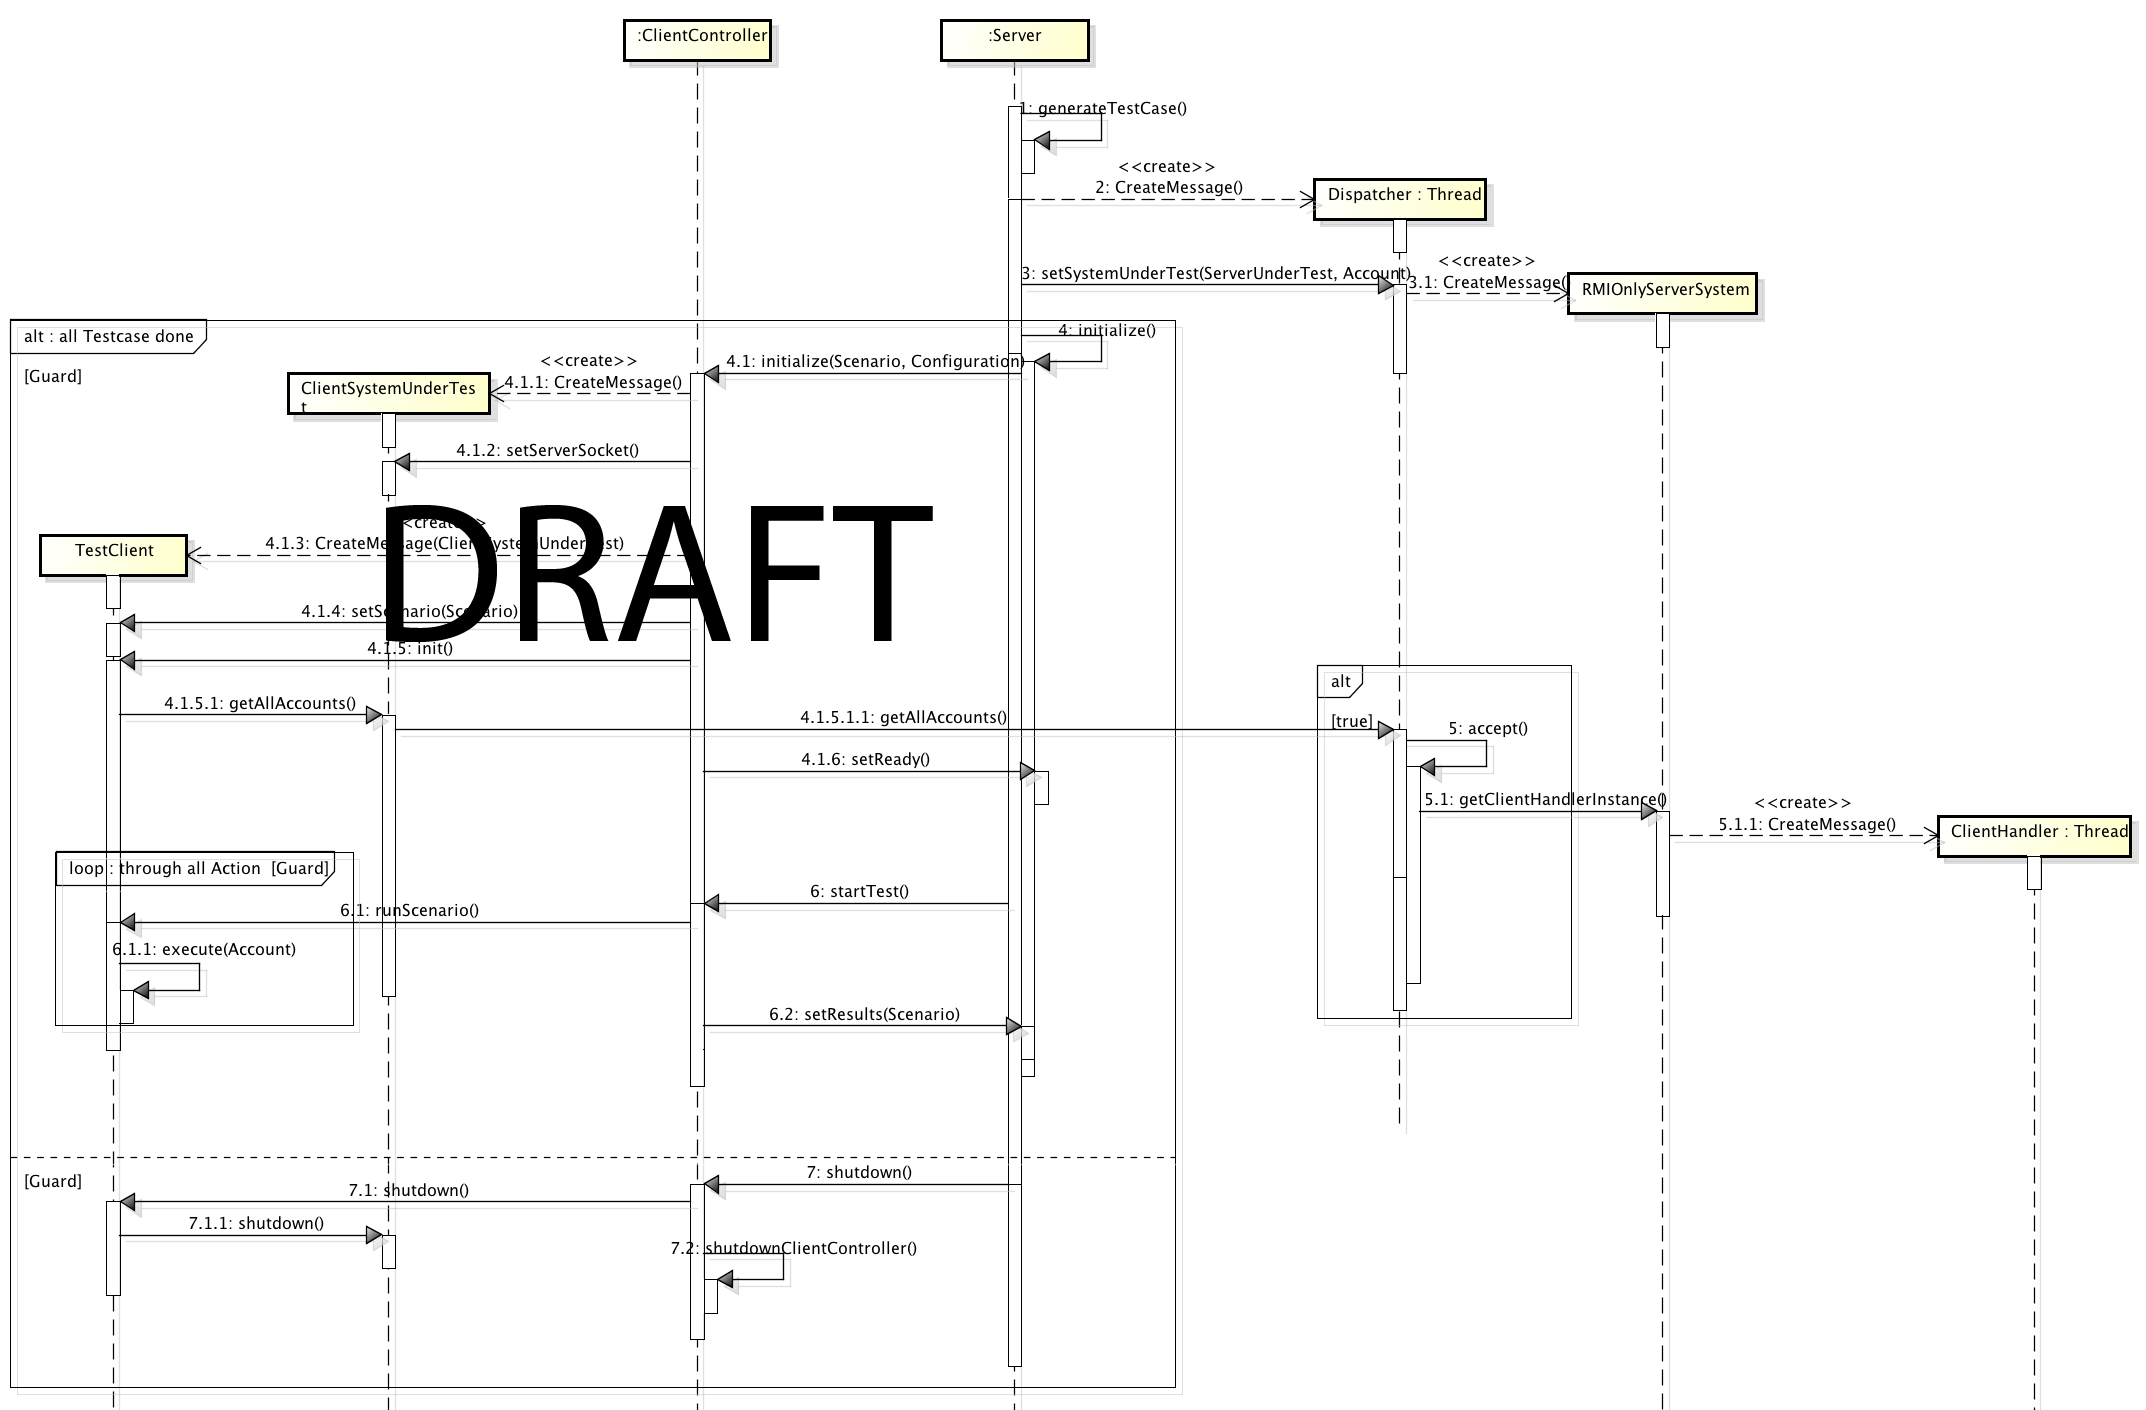
\includegraphics[scale=0.2]{image_testFramework/TestFWServerClientSeq.png}
\end{center}
\caption{Server Client Communication}
\end{figure}
 
Beim Start der client.jar Datei kann das Startup-Skript zwei Argumente mitgeben:
\begin{enumerate}
\item Binding Namen
\item Optional: ein RMI-Port
\end{enumerate}
Die Kommunikation zwischen dem Testframework Client und dem Server ist über Java RMI realisiert. Der Startvorgang sieht wie folgt aus:
\begin{itemize}
\item Es wird ein neues ClientController Objekt instanziiert. Der ClientController implementiert das Client Interface, welches von Remote ableitet.
\item Daraufhin wird aus dem neue ClientController Objekte ein Remoteobjekt erzeugt.
\item Der lokale Name Service wird auf dem optionalen Port gestartet, ist kein Port spezifiziert wird der Defaultport 1099 verwendet.
\item Das ClientController Remoteobjekt lässt sich nun in dem Java Name Service unter dem Binding Name veröffentlichen. Nun kann der Server eine ClientController Stub lokalisieren und somit den ClientController über RMI steuern.
\end{itemize}

Über folgendes Remote Interface wird der ClientController konfiguriert und gesteuert:
\begin{lstlisting}[language=java, breaklines=true] 	
public void initialize(Scenario scenario, Configuration configuration) throws RemoteException;
public void startTest() throws RemoteException;
public void shutdown() throws RemoteException;
\end{lstlisting}
Die Grundidee zu Beginn des Projekts war, dass alle Konfigurationswerte einzeln als Parameter an den ClientController übergeben werden. Es stellte sich jedoch schnell heraus, dass eine Kappselung der benötigen Parameter in einem seperaten Objekt eine wesentlich bessere Lösung darstellt. Dieses neue Datatransfer Object, beinhaltet sowohl alle nötigen Parameter für die Konfiguration des ClientSystemUnderTest sowie des ClientControllers. Der Name des ClientSystemUnderTest, sowie die Informationen für den erfolgreichen Aufbau eines RMI Kommunikationkanals zwischen dem Testframework Client und dem Testframework Server, sind in diesem Objekt hinterlegt.

\subsubsection{Initialize des ClientControllers}
In der konkreten Implementation der Methode "initialize(Scenario scenario, Configuration configuration)" werden mehrer Aufgaben erledigt:
\begin{enumerate}
\item Aus dem Configuration Objekt wird die Server IP, der RMI Port und der Name unter dem der Server registriert ist ausgelesen. Aus diesen Information wird eine neue RMI Verbindung zum Server erzeugt.
\item Die Instanziierung des konkreten ClientSystemUnderTest übernimmt eine einzlne Klasse, welche als Factory implementiert ist. Der Factory wird nur der "fully qualified name", welcher im Configuration Objekt gespeichert ist, übergeben. Die Factory selbst instanziiert den ge\-wünschten Client\-System\-Under\-Test via Re\-flec\-ti\-on und re\-turniert dieses.
\item Auf dem ClientSystemUnderTest wird nun ein neues Socket, welches zum ServerSystemUnderTest zeigt, gesetzt.
\item Ein neuer TestClient wird erzeugt und das aktuelle ClientSystemUnderTest Objekt wird im Konstruktor mitgegeben. Der TestClient ist die Schnittstelle zwischen dem ClientController und dem ClientSystemUnderTest.
\item Nun wird dem TestClient das Scenario übergeben und der TestClient initialisiert
\item Der TestframeworkServer wird über die erfolgreiche Konfiguration, des ClientControllers und des ClientSystemUnderTest informiert. Über die zu Beginn erzeugte RMI Verbindung wird nun "setReady()" auf dem Server aufgerufen.
\item Der ClientController wartet, bis der Server den Test startet.
\end{enumerate}

\subsubsection{Start eines Testlaufs}
Der Server startet den Testdurchlauf parallel auf allen ClientController über die Methode "startTest()". Diese ruft auf dem TestClient "runScenario()" auf, eine detailierte Erklärung was in dieser Methode passiert, ist im Kapitel "Test Client" zu finden. Sind alle Aktionen des gegeben Szenarios abgearbeitet, wird das gesamte Szenario mit den enthaltenen Messresultaten über die Methode "setResults(Scenario scenario, String IP)" zurück an den Server geschickt.

\subsubsection{Herunterfahren des Clients}
Die Methode "shutdown()" be\-endet den Test\-framework\-Client und das Client\-System\-Under\-Test. Die shutdown() Methode besteht aus mehreren Teilschritten:
\begin{enumerate}
\item Die Verbindung zwischen dem spezifischen Namen und dem damit verbundenen ClientController Remoteobjekt wird im Name Service von Java gelöscht.
\item Das ClientController Objekt wird von der RMI Run\-time entfernt, da\-durch sind keine RMI Aufrufe mehr möglich.
\item Der ClientController beendet sich selbst
\end{enumerate}


Beim Testen der shutdown()-Funktionalität konnte festgestellt werden, dass bei der Umsetzung wie oben beschrieben, der Server immer eine Exception bekommt. Es stellte sich heraus, dass das sofortige Herunterfahren des ClientControllers nach dem Unbinding und dem Unexport dem Server keine Zeit lässt, seine RMI Verbindung zum ClientController korrekt zu schliessen. Die Lösung dieses Problems lag, in einem verzögerten Herunterfahren des ClientControllers. Folgender Codeausschnitt zeigt die Lösung des Problems.
\begin{lstlisting}[language=java, breaklines=true]
private void closeClientController(final long delay) {
new Thread() {
	@Override
	public void run() {
		logger.info("ClientController is shutting down");
		try {
			sleep(delay);
		} catch (InterruptedException e) {
		}
		System.exit(0);
		}
	}.start();
}
\end{lstlisting}
Die Beendigung des ClientControllers wird in einem seperaten Thread ausgeführt, so\-dass der Main- Thread noch ge\-nü\-gend Zeit hat, alle of\-fe\-nen Ver\-bin\-dun<-gen ord\-nungs\-gemäss zu schliessen. Der shutdown Thread beendet den ClientController nach der mittels "delay" mit\-ge\-ge\-be\-nen Zeit\-span\-ne mit System.exit().   

\subsection{Test Client}
\label{sec:testclient}

\begin{figure}[H]
\begin{center}
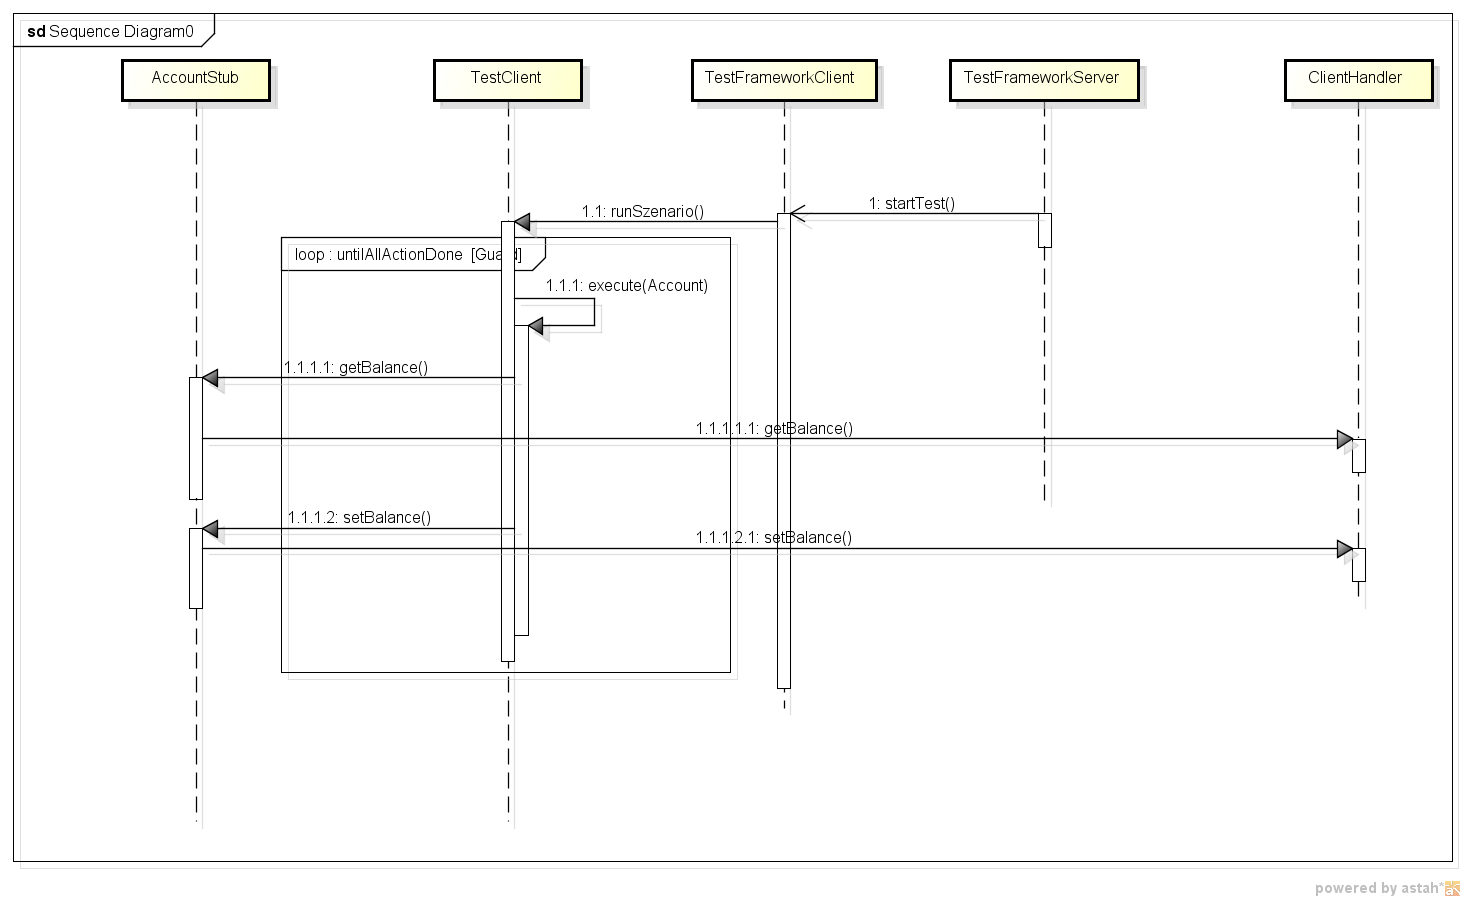
\includegraphics[scale=0.3]{image_testFramework/startTest.png}
\end{center}
\caption{start Tests}
\end{figure}

Die TestClient Klasse ist die Schnittstelle zwischen dem ClientController und dem ClientSystemUnderTest. Das Interface ClientSystemUnderTest ist die  Schnittstelle die alle ClientSystemUnderTest Clients implementieren müssen, so lassen sich alle Varianten von ClientSystemUnderTest über diesen TestClient testen. Desweiteren kann auf dem TestClient das Szenario gesetzt werden, welches der TestClient beim Aufruf von "runScenario()" durch den ClientController abarbeitet.

Das ClientSystemUnderTest Interface ist wie folgt definiert:
\begin{lstlisting}[language=java, breaklines=true] 	
public interface ClientSystemUnderTest {	
	public AccountService getAccountService();
	public void setServerSocketAdress(InetSocketAddress socketAdress);
	public void shutdown();
}	
\end{lstlisting}
\subsubsection{Ablauf}
\label{sec:ablauf}
\begin{itemize}
\item Der ClientController setzt die Socket Adresse des Server in das Client\-System\-Under\-Test. Die nötigen Imformationen sind ebenfalls im Configuration Objekt gespeichert.
\item Im Konstruktor des TestClients wird der AccountService, des über\-gebenen ClientSystemUnderTest über die Meth\-ode "getAccountService()" geladen. 
\item Während der Initialisierungs- Phase des ClientController ruft dieser ebenfalls die "init()" Methode des TestClients auf, dadurch wird eine Liste aller Accounts Objekte aus dem AccountService in den TestClient geladen.
\item Startet der Server nun den Testlauf wird endlos durch die Liste der Accounts interiert bis alle Aktionen des gesetzten Szenarios abgearbeitet sind.
\item Bei einem Shutdown durch den Server ist der TestClient ebenfalls für die ord\-nungs\-ge\-mä\-sse Be\-en\-di\-gung des ClientSystemUnderTest zu\-stän\-dig.
\end{itemize}

\subsubsection{Concurrency im TestClient}
\label{sec:concurrencyTestClient}
Während der ersten Testmessungen mit den Cache- System zeige sich folgendes Problem. Der letzte TestClient, der sich beim Server als bereit meldet, benötigte für die ersten Aktionen im Durchschnitt etwa 40 Milisekunden länger als die restlichen Clients. Durch die Analyse des Codes konnte folgender Ablauf rekonstruiert werden:
\begin{enumerate}
\item Der letzte Client meldet seine "setReady()" Status dem Server. Dabei besteht der Thread auf dem Client weiter, bis der "setReady()" Aufruf auf dem Server zurückkehrt.
\item Auf dem Server wird beim Aufruf der "setReady()" Methode ein neuer Thread vom RMI Daemon erzeugt. Dieser Thread prüft in der Methode, ob alle Clients nun sind. Diese Bedingung trifft nun ein, daher wird auf jedem Client die "startTest()" Methode aufgerufen und die Messung beginnt.
\item Während dessen wartet der Client\-Controller Thread immer noch auf die Rückkehr des "setReady()" Aufrufs, während auf allen Clients zur gleichen Zeit die "startTest()" Methode aufgerufen wird, dadurch existieren beim letzten Client, der sich beim Server meldet, kurz\-zeitig zwei Threads. Neben des "set\-Ready()" Thread läuft der "start\-Test()" Th\-read eben\-falls und be\-ginnt mit der Ab\-ar\-bei\-tung des Sze\-nar\-ios. Kehrt nun der "set\-Ready()" Th\-read zu\-rück, be\-endet sich dieser Th\-read. Die CPU- Res\-sour\-cen werden da\-rauf\-hin dem "startTest()" Thread in der Anfangs\-phase der Aktion weg\-ge\-nommen und für die Be\-endi\-gung des "setReady()" Threads benötigt. Dies führt nun zu einer Verlängerung der Ausführungsdauer der Aktion.
\end{enumerate}
Die Lösung dieses Problem lag in einer Wartephase vor dem eigentlichen Abarbeiten des Szenarios. Diese Pause wurde über Thread.sleep() umgesetzt und wird vor der eingentliche Messung gemacht. Dadurch haben alle ClientController Zeit, den "setReady()" Thread zu beenden, ohne den "startTest()" Thread zu beeinträchtigen.



\subsection{Action}
\label{sec:action}
Ein Szenario beinhaltet eine Menge von Aktionen, welche auf ein Account Objekt ausgeführt werden können. Für eine einfache Erweiterbarkeit von neuen Aktionen, ist hierfür das Command-Pattern benutzt worden. Alle konkreten Implementierung einer Aktion müssen von der abstrakte Klasse Action ableiten. Im Konstruktor dieser abstrakten Klasse wird ein neues Result Objekt(siehe Kapitel Result) instanziert. Dieses Objekt dient als Datenkontainer für alle Zeitmessungen die während dieser Aktion gesammelt werden sollen. Desweiteren deklariert Action drei abstrakte Methoden die von Subklassen implementiert werden müssen.
\begin{lstlisting}[language=java, breaklines=true] 	
public abstract ActionTyp getActionTyp();
public abstract int getMinimalNumberOfTimeRecords();
public abstract void execute(Account account);	
\end{lstlisting}

\begin{itemize}
\item Für eine detailierte Auswertung muss der Typ der Aktion zugänglich gemacht werden, dies ist über die Methode "getActionTyp()" möglich.
\item Eine Aktion besteht aus einer Abfolge von "getBalance()" und "setBalance(double value)" Aufrufen. Jenach Aktion können mehrer Methodenaufrufe auf das Account Objekt nötig sein um die Aktion erfolgreich auszuführen. Um im Reporting festzustellen ob die ganze Aktion beim ersten Versuch erfolgreich war, muss die minimale Anzahl von TimeRecords, die für den Erfolg der Aktion nötig sind, über die Methode "getMinimalNumberOfTimeRecords()" zugänglich gemacht werden. So lassen sich Konflikte, die bei der Ausführung dieser Aktion auftreten, im Reporting feststellen.
\item Die Methode "execute(Account account)" beinhaltet die eigentliche Aktion die auf dem Account-Objekt ausgeführt werden soll.
\end{itemize} 

\subsection{ActionTyp}
\label{sec:actionTyp}
Der ActionTyp wird zur Indentifizierung der Aktion benutzt und ist als Enum realisiert. Folgende Aktionstypen sind bereits vorhanden:
\begin{itemize}
\item ReadAction
\item WriteAction
\item IncrementAction
\end{itemize}
Die Werte dieses Enums werden zur Erkennung des Aktiontyps genutzt und wird bei der Report Generierung verwendet.

 
\subsection{Increment Action}
\label{sec:incrementAction}
Die Aktion Kontostand-Erhöhen (IncrementAction) ist die Kernaktion für alle Szenarien. 
Sie besteht aus drei Teilschritten:
\begin{itemize}
\item Aktuellen Kontostand über die Methode "getBalance()" aus dem Account holen und zwischenspeichern
\item Den temporären Kontostand mit dem gegeben Faktor multiplizieren
\item Versuchen den neuen Wert via "setBalance(double value)" Methode zurück in das Konto, welches auf dem Server liegt, zu schreiben. 
\end{itemize}

\begin{lstlisting}[language=java, breaklines=true] 
@Override
public void execute(Account account) {
	boolean successful = false;
	double balance = 0;
	int numberOfTry = 0;
	while (!successful) {
		result.startTimeMeasurement(BasicAction.READ);
		balance = account.getBalance();
		result.stopTimeMeasurement();
		sleep(numberOfTry);
		try {
			result.startTimeMeasurement(BasicAction.WRITE);
			account.setBalance(balance * factor);
			result.stopTimeMeasurement();
			successful = true;
		} catch (RuntimeException e) {
			successful = false;
			result.stopTimeMeasurement(ActionResult.FAILED);
		}
		numberOfTry++;
	}
}
\end{lstlisting}
Im Laufe der Rea\-li\-sie\-rung stellte sich her\-aus das zwi\-schen dem "get\-B\-alan\-ce()" und dem "set\-Ba\-lan\-ce()" Auf\-ruf eine mi\-ni\-mal de\-fi\-nier\-ba\-re Zeit\-dauer ge\-wartet werden können muss. Diese Warteperiode ist nötig, damit sich leichter ein Konflikt erzeugen lässt und so gezeigt werden kann, dass der Fehler serverseitig zu keinem Lost-Updates führt.
\newline
Tritt serverseitig ein Concurrency Fehler auf, wird eine RuntimeExeption zurück an den Client geworfen. Dieser Fehler führt dazu, dass die Aktion nochmals neu gestartet wird. Die Aktion wird solange wiederholt bis diese erfolgreich aus der While-Schleife kommt. Die Verzögerung zwischen dem Lesen und Schreiben, welche über die Methode "sleep()" realisiert ist, führt nur beim ersten Versuch der IncrementAction zu einer zeitlichen Verzögerung.


Dies veranlasst die Aktion dazu, dass sie mit der kom\-p\-le\-te Aktion noch\-mals neu beginnt, mit dem Unterschied, das diesmal keine Verzögerung zwischen getBalance() und setBalance() benutzt wird. Dies wird über den Wert numberOfTry geprüft, ist dieser grösser als eins wird die Verzögerung nicht nochmals ausgeführt.

\subsection{WriteAction}
\label{sec:writeAction}
Die WriteAction wurde nur zu Beginn der Realisierung benutzt und schreibt via "setBalance()" auf einem Account einen gegeben Wert. 

\subsection{ReadAction}
\label{sec:readAction}
Die WriteAction wurde ebenfalls nur zu Beginn der Realisierung benutzt. Diese Aktion liest den aktuellen Kontostand eine Objekts und speichert diesen ab. Über "getBalance()" kann auf den Kontostand zugegriffen werden.

\subsection{Result}
\label{sec:result}
Für die möglichst genaue Zeitmessung einer Aktion wird die von Java bereitgestellte Methode System.nanoTime() genutzt. Die Klasse Result bietet eine "startTimeMeasurement(BasicAction type)" Methode die ein neues TimeRecord Objekt erzeugt und die momentane Zeit in dieses TimeRecord Objekt schreibt. Die Information, ob es sich bei dieser Messung um eine lesende oder schreibende Methode handelt wird über denn BasicAction-Typ an den TimeRecord weiter gegeben. Diese ist nötig, damit bei der Auswertung genau analysiert werden kann, für welchen Methodeaufruf (getBalance() / setBalance()) dieser TimeRecord erzeugt wurde. Über die Methode "stopTimeMeasurement(ActionResult result)" lässt sich die Zeitmessung beenden und der aktuelle TimeRecord wird in einer Liste gespeichert. Das Argument, welches in der "stopTimeMeasurment()" Methode übergeben wird beinhaltet die Information über den Erfolg der Aktion. So lassen sich auch Aktionen erzeugen die aus mehreren setBalance() oder getBalance() Aufrufe bestehen. Dies ist zum Beispiel in der IncrementAction der Fall.

\subsection{TimeRecord}
\label{sec:timeRecord}
Der TimeRecordtyp ist als reines Data Tranfer Object implementiert worden. Es beinhaltet die Startzeit sowie die Stopzeit genau eines Methoden Aufrufs. Für eine genaue Auswertung einer Aktion sind noch weitere Daten nötig. Daher besitzt dieser Typ zwei weitere Felder. Der BasicActiontyp beinhaltet Informationen für welche Account Methode, also getBalance oder setBalance, dieser Record gilt und in dem ActionResult kann die Information über den Erfolg der BasicAction gespeichert werden. Dadurch lassen sich zusammengesetzte Aktionen, welche aus getBalance() und setBalance() zusammengesetzt sind einfach unterteilen.

\subsection{BasicAction}
\label{sec:BasicAction}
Damit eine genaue Analyse der Aktionen ge\-macht werden kann, ist es nö\-tig, dass zwi\-schen "get\-Ba\-lan\-ce()" und "set\-Ba\-lan\-ce()" un\-ter\-schieden wer\-den kann. Eine Aktion kann aus mehreren Methoden\-auf\-rufen bestehen, daher muss bei einer Zeitmessung die Art(setter / getter) angegeben werden können. Da jedoch eine Aktion aus einer Abfolge von Reads und Writes bestehen kann, ist es nötig, dass diese Information gespeichert wird. Im TimeRecord lässt sich daher die BasicAction speichern.

\subsection{ActionResult}
\label{sec:ActionResult}
Den Erfolg eines getBalance() oder setBalance() Aufrufs lässt sich ebenfalls im TimeRecord speichern. Um eine Statistik über die Fehlerrate beider Methodenaufrufe zu bekommen, war es daher nötig, dass beim stoppen einer Messung, der eine BasicAction zugrunde liegt den Erfolgstatus gespeichert werden kann. Damit lässt sich ein Szenario auf die zwei Grundoperation setBalance() und getBalance() herunterbrechen. Dies ermöglicht es die Auswertung bis auf diese zwei Methoden hinab zu analyisieren und auszuwerten.

